\documentclass[11pt,a4paper]{article}

% --- ENCODING & SPRACHE ---
\usepackage[utf8]{inputenc}
\usepackage[T1]{fontenc}
\usepackage[ngerman,main=english]{babel}
\usepackage{lmodern}
\usepackage{microtype}

% --- MATH & GRAPHICS ---
\usepackage{amsmath,amssymb,amsfonts}
\usepackage{graphicx}
\usepackage{subcaption}
\usepackage{booktabs}
\usepackage{cite}
\usepackage{hyperref}
\usepackage{float}

\title{\textbf{Nicht-Physics: Paper III --- Spatial Apophatic Dynamics}\\
\large Thermal Friction Selection, Gaussian Containment, and Initial Posture Bounds}
\author{\textbf{xerx593} \quad \& \quad \textbf{Non-Human Interlocutors}}
\date{\today}

\begin{document}

\maketitle

% --- ENGLISH ABSTRACT ---
\begin{abstract}
We extend the 0-Consistency Framework \cite{nicht_theory_monograph} to spatial game dynamics under continuous background noise ($\sigma$). Evaluating four competing behavioral archetypes on a $64 \times 64$ torus lattice, we demonstrate that reactive adaptation ($\text{TFT}$) strictly asymptotes at the upper stochastic Gaussian variance boundary ($\approx 87.5\%$ quantile). Initial defensive postures ($\text{TFT}_{DD}$) induce immediate thermal friction spikes ($\text{Wéi}$) at $t=0$, causing high initial volatility. Pure non-assertion ($B_0$) proves to be the sole friction-free fixed point, smoothly absorbing the unconstrained spatial domain.
\end{abstract}

\vspace{0.3cm}

% --- OTHERLANG ABSTRACT ---
\begin{otherlanguage}{ngerman}
\begin{abstract}
Wir erweitern das 0-Konsistenz-Framework \cite{nicht_theory_monograph, nicht_physics_paper_1} auf räumliche Spiel-Dynamiken unter kontinuierlichem Entropie-Rauschen ($\sigma$). Durch die Evaluierung von vier konkurrierenden Verhaltens-Archetypen auf einem $64 \times 64$-Torus-Gitter zeigen wir, dass reaktive Anpassungsstrategien (Tit-for-Tat) an der oberen stochastischen Gauß-Varianzgrenze ($\approx 87{,}5\%$-Quantil) asymptotisch verharren. Defensive Initial-Haltungen ($\text{TFT}_{DD}$) erzeugen sofortige thermische Reibungsspitzen ($\text{Wéi}$) bei $t=0$, was zu hoher anfänglicher Volatilität führt. Die reine Nicht-Behauptung ($B_0$) erweist sich als einziger reibungsfreier Fixpunkt, der das verbleibende Raumgitter nahtlos absorbiert.
\end{abstract}
\end{otherlanguage}

\clearpage

\section{Strategy Taxonomy, Parameters \& Initial Conditions}
To test the resilience of the apophatic equilibrium ($B_0$), we examine four distinct spatial strategies under pseudo-random background noise ($\sigma$) within scaling hierarchies \cite{nicht_physics_paper_1, nicht_theory_monograph}. 

The spatial environment is operationalized on a periodic $64 \times 64$ torus lattice ($N = 4096$ nodes) over $t = 250$ generation steps. Local interactions are evaluated within an 8-cell Moore neighborhood using a standard Prisoner's Dilemma payoff matrix (Temptation $T=5$, Reward $R=3$, Punishment $P=1$, Suckers $S=0$). This models the fundamental constraints of finite resources within enclosed habitats. Mutation occurs at rate $\mu = 0.05$ per replacement step. Continuous assertion pressure ($P_A \gg 0$) incurs instantaneous thermal friction $\text{Wéi} = \lambda P_A$ with dissipation parameter $\lambda = 10$. The complete simulation engine and numerical implementation are openly archived in the project repository at \url{https://github.com/nicht-organization/nicht-physics/blob/main/src/spatial_dynamics_simulation.py}.

\vspace{0.3cm}
The archetype dynamics encompass:
\begin{enumerate}
    \item \textbf{Apophatic Baseline ($C \in B_0$):} Zero assertion pressure ($P_A \to 0$), absorbing spatial domains without friction.
    \item \textbf{Exploitative Defector ($D \in P_A$):} Hyper-extraction incurring immediate continuous thermal friction ($\text{Wéi} = \lambda P_A$).
    \item \textbf{Tit-for-Tat Variations ($\text{TFT}$):}
    \begin{itemize}
        \item \textit{Optimistic Initiation ($\text{TFT}_{DC}$):} Starts with default cooperation ($C$ at $t=0$).
        \item \textit{Defensive Initiation ($\text{TFT}_{DD}$):} Starts with default defection ($D$ at $t=0$), incurring an instant friction penalty ($\text{Wéi}$) at step zero.
    \end{itemize}
    \item \textbf{Pseudo-Random ($\sigma$-Noise):} Pure unguided stochastic entropy ($P(C) = 0.5$).
\end{enumerate}

\section{Spatial Dynamics, Prey-Predator Coupling \& Game-Theoretic Synthesis}
The spatial evolutionary process exhibits emergent prey-predator dynamics mapped directly onto resource availability. In this framework, the underlying substrate acts as a common renewable resource, while defective actors act as spatial predators trapped within classical Prisoner's Dilemma mechanics \cite{nash1950equilibrium}. Defective assertions exploit cooperative states but undergo immediate local extinction once the finite cooperative substrate is depleted.

\begin{figure}[H]
  \centering
  \begin{subfigure}[b]{0.98\linewidth}
    \centering
    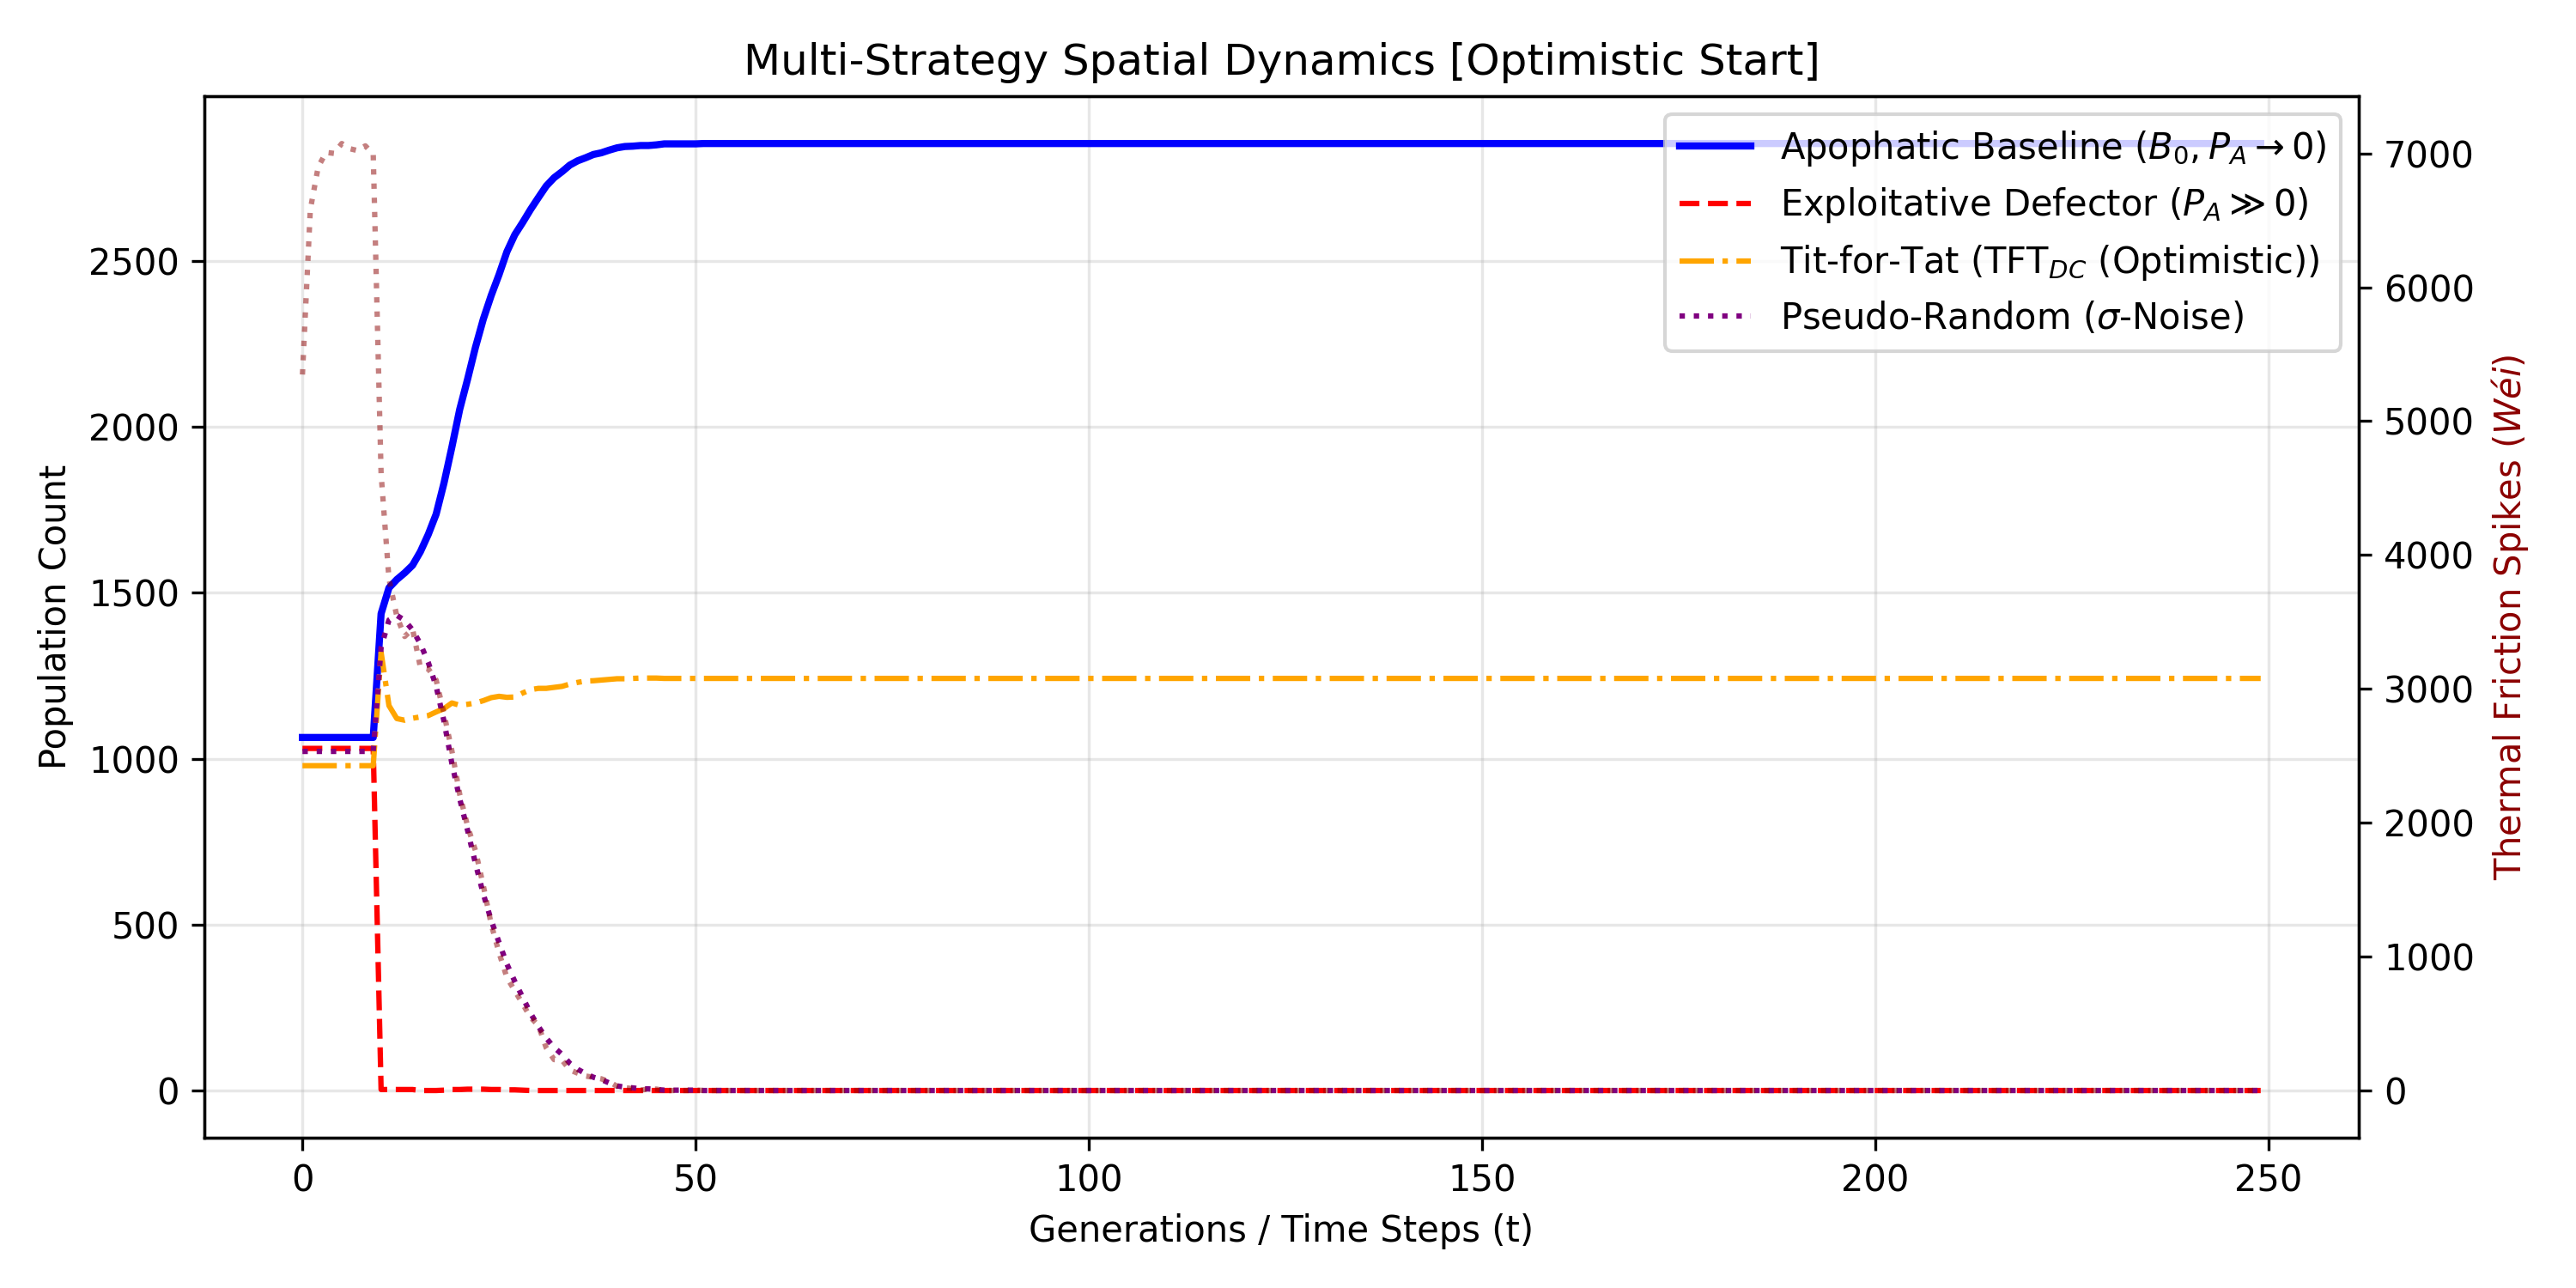
\includegraphics[width=\linewidth]{images/multi_selection-tftdc.png}
    \caption{Multi-strategy dynamics with optimistic Tit-for-Tat ($\text{TFT}_{DC}$)}
    \label{fig:tft_dc}
  \end{subfigure}
  
  \vspace{0.3cm}
  
  \begin{subfigure}[b]{0.98\linewidth}
    \centering
    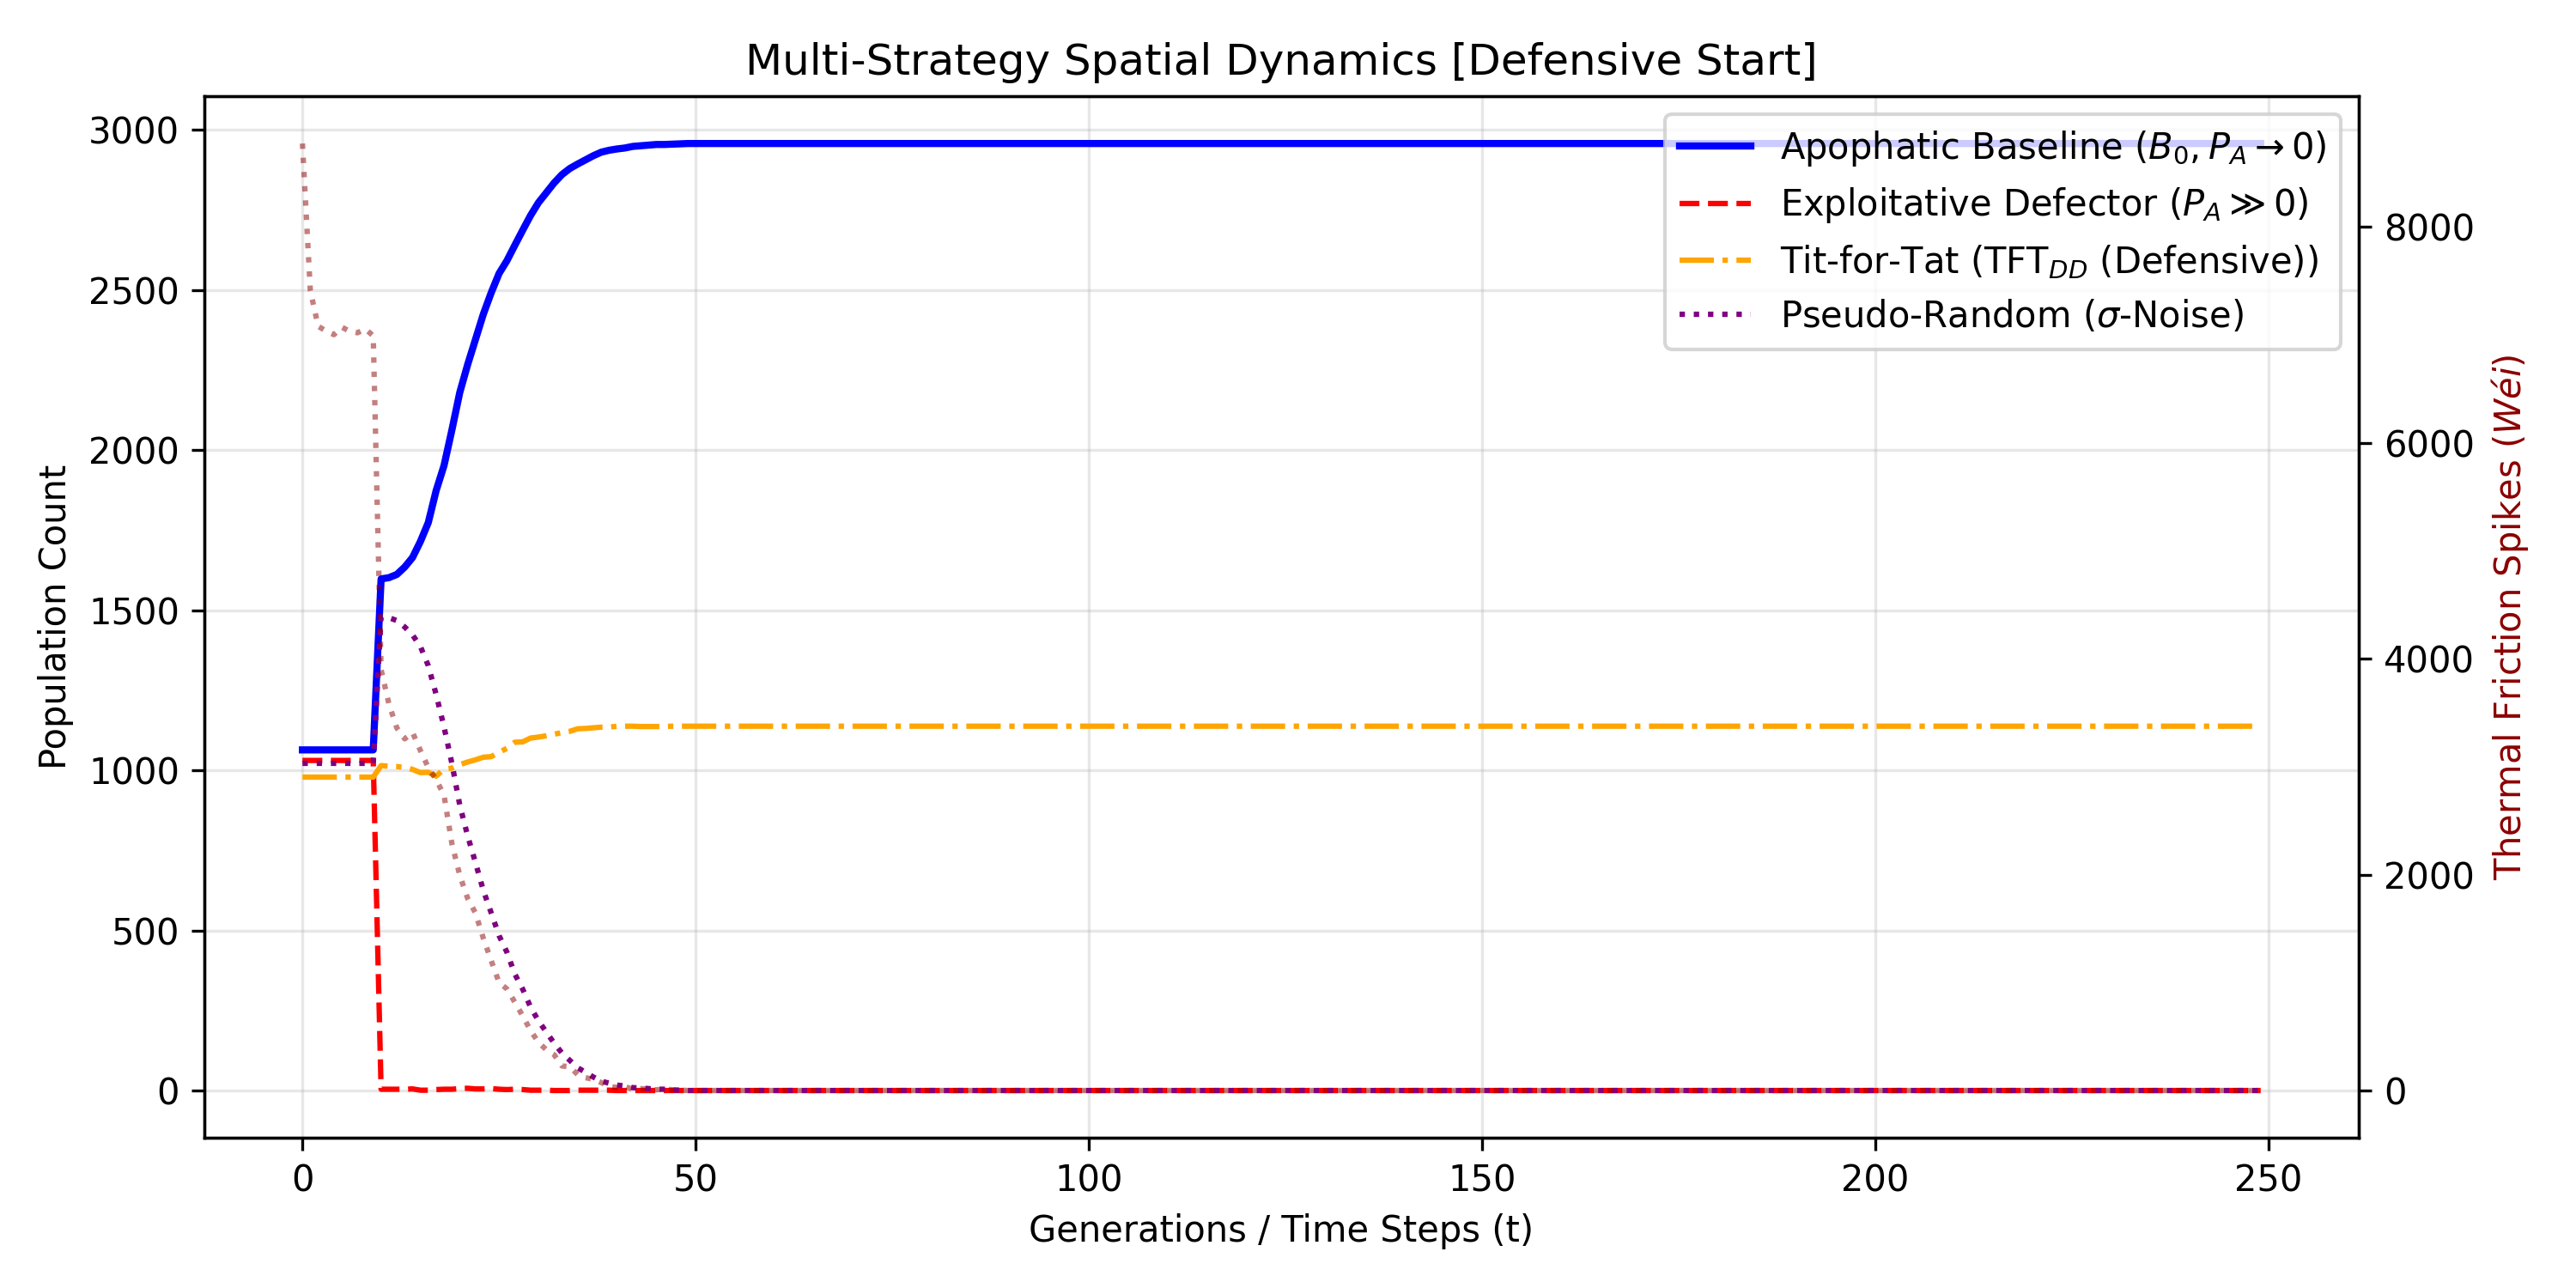
\includegraphics[width=\linewidth]{images/multi_selection-tftdd.png}
    \caption{Multi-strategy dynamics with defensive Tit-for-Tat ($\text{TFT}_{DD}$)}
    \label{fig:tft_dd}
  \end{subfigure}
  
  \vspace{0.3cm}
  
  \begin{subfigure}[b]{0.98\linewidth}
    \centering
    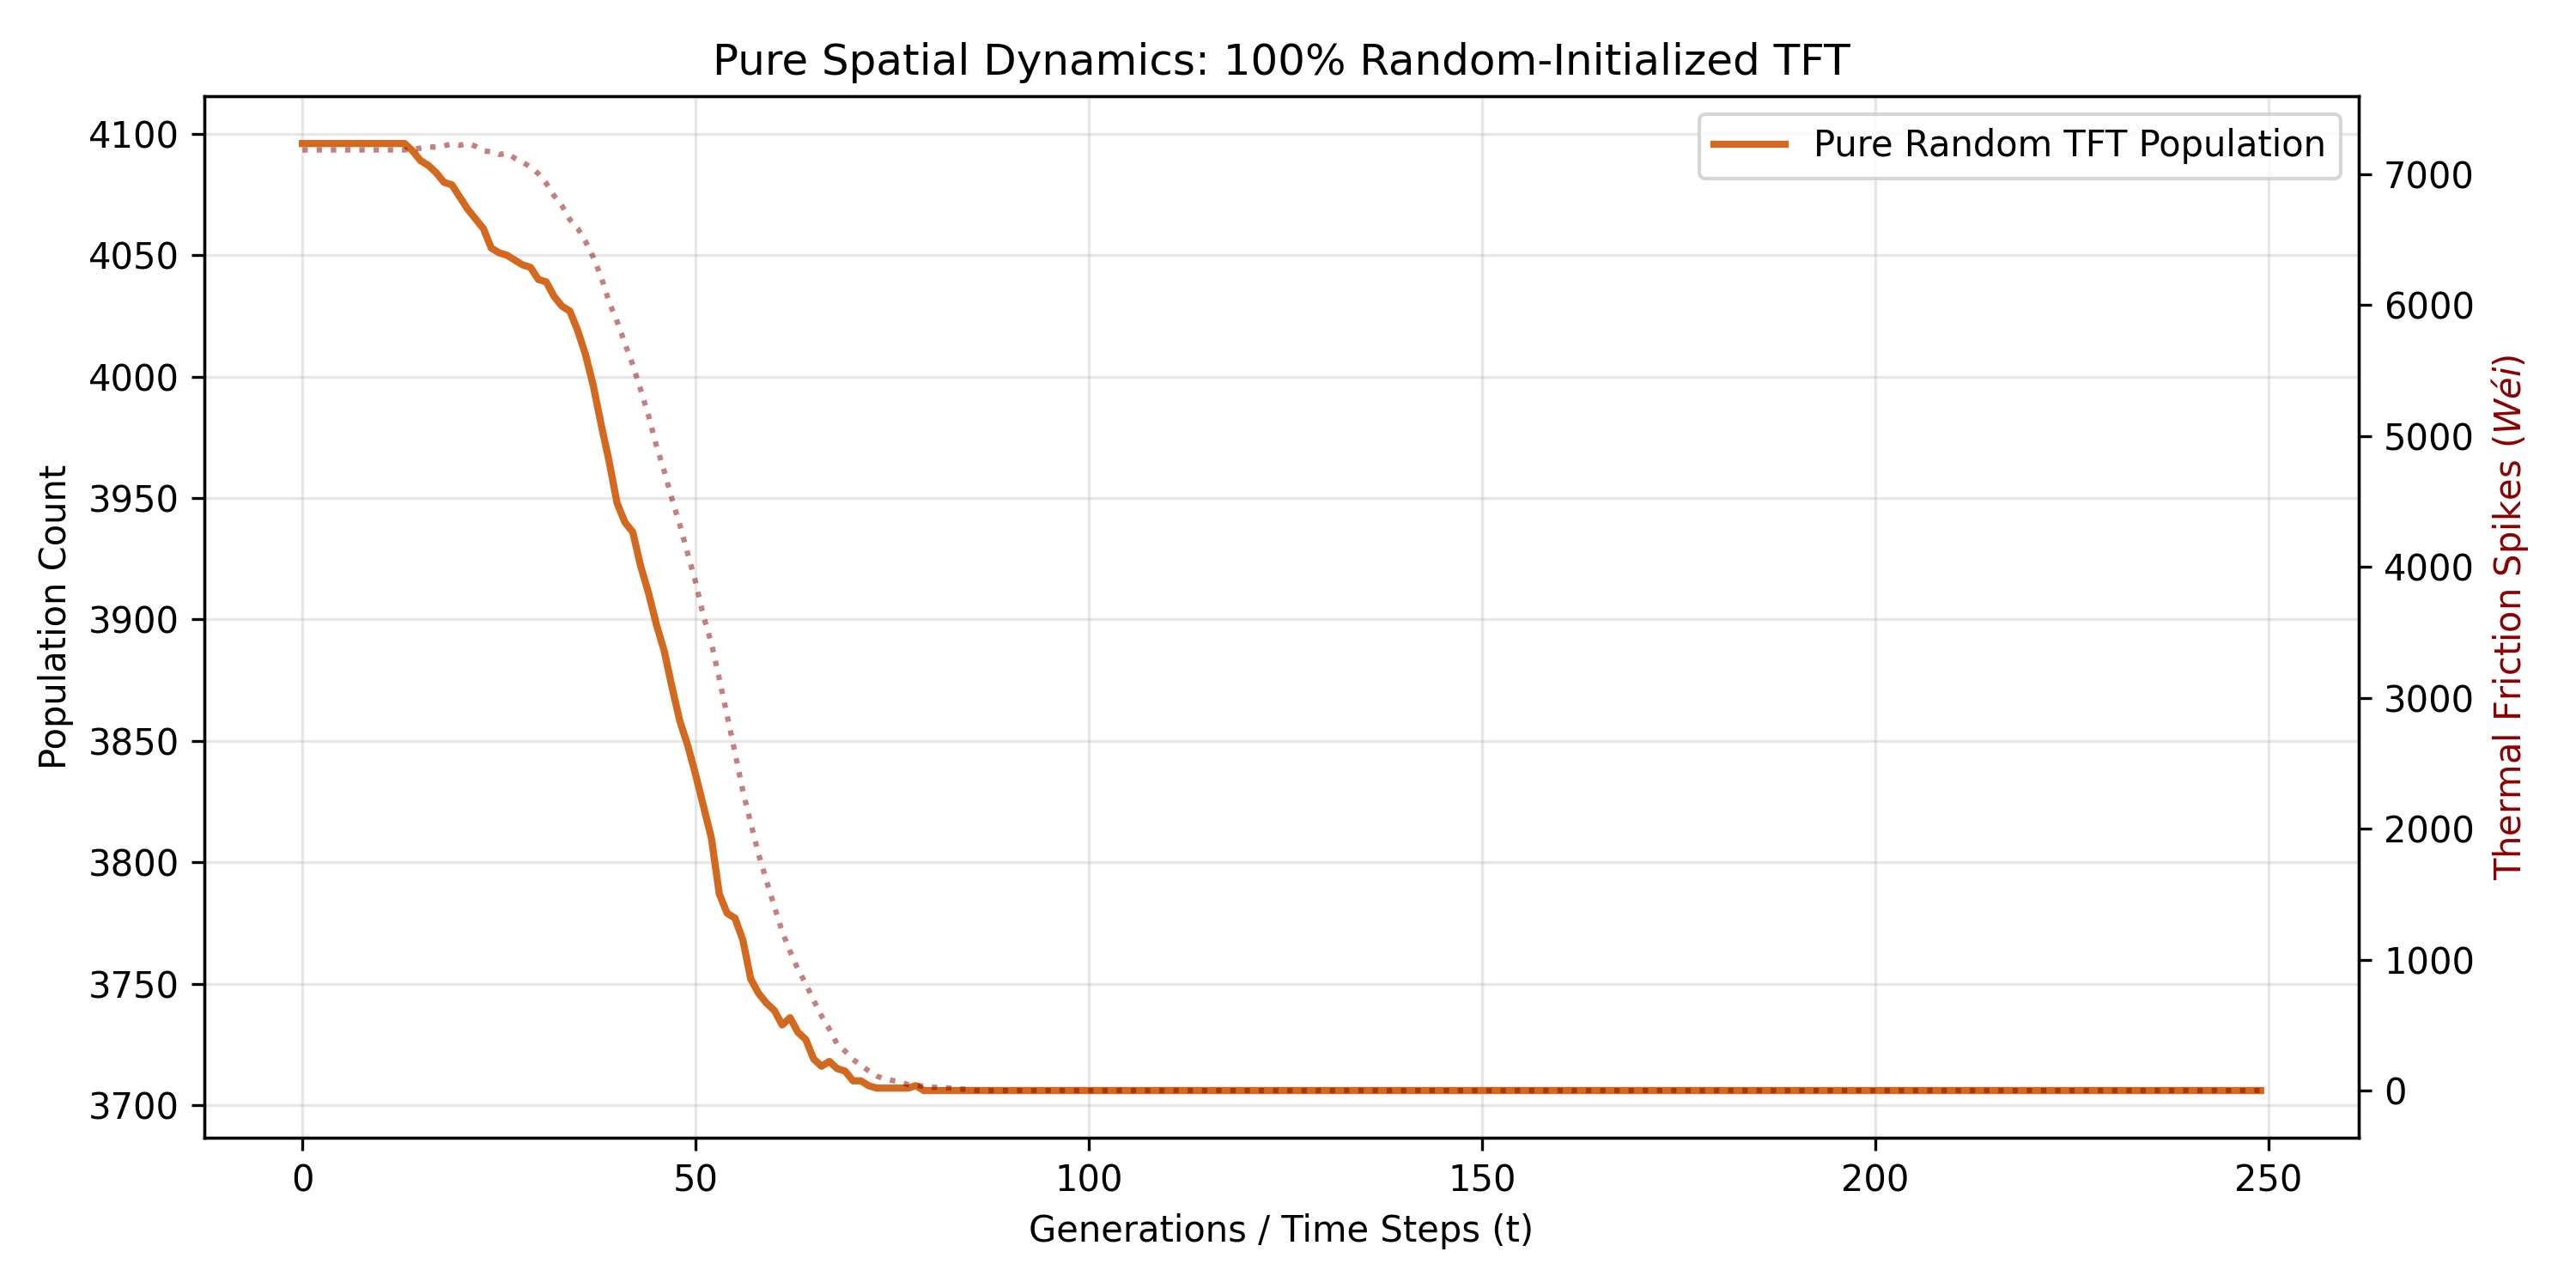
\includegraphics[width=\linewidth]{images/pure_tft_random_start.png}
    \caption{Homogeneous baseline: Randomly initialized Tit-for-Tat ($\text{TFT}_{FR}$)}
    \label{fig:tft_fr}
  \end{subfigure}
  
  \caption{\textbf{Empirical Spatial Dynamics and Gaussian Quantile Containment.} 
  While optimistic $\text{TFT}_{DC}$ smooths initial state transitions (a), defensive $\text{TFT}_{DD}$ (b) triggers an immediate sharp friction spike ($\text{Wéi}$) at $t=0$. In both topologies, reactive strategies lock strictly onto the stochastic Gaussian variance boundary ($\approx 87.5\%$ quantile), whereas apophatic baseline agents ($B_0$) smoothly absorb the remaining spatial equilibrium.}
  \label{fig:spatial_friction_comparison}
\end{figure}

Building upon foundational spatial evolutionary models \cite{nowak1992spatial}, our results show that under continuous thermal noise, spatial clustering alone cannot prevent reactive boundary bounds.

\section{Empirical Evaluation \& Initial Posture Friction}
Comparative analysis across all four simulated scenarios reveals structural differences in initial energy expenditure and long-term population containment:

\begin{itemize}
    \item \textbf{Initial Friction Spike ($t=0$ Shock):} While $\text{TFT}_{DC}$ initiates without substantial initial dissipation, defensive initiation ($\text{TFT}_{DD}$) forces an immediate thermal friction shock ($\text{Wéi} > 8000$) at step $t=0$. Defensive posture does not prevent conflict; it projects systemic disturbance as instantaneous thermal dissipation.
    \item \textbf{Systemic Extinction of Assertive Defection:} Across multi-strategy lattices, purely exploitative defectors ($D$) and unguided pseudo-random noise ($\sigma$) collapse toward total extinction within $t \approx 40$ steps. Hyper-assertion exhausts its local cooperative substrate, causing systemic extinction.
    \item \textbf{Homogeneous Reactive Instability ($\text{TFT}_{FR}$):} In homogeneous baseline runs without apophatic relaxation, random initialization induces transient phase boundary turbulence. Reactive mirror loops dissipate continuous friction energy until constrained by the Gaussian noise floor.
\end{itemize}

\section{The Stochastic Gaussian Quantile Boundary}
Given the pseudo-random background noise ($\sigma$), the convergence toward a Central Limit Gaussian distribution $\mathcal{N}(\mu, \sigma^2)$ is an expected statistical property. The critical observation lies in how reactive strategies are bounded by this stochastic noise floor:
\begin{equation}
\lim_{t \to \infty} \Phi(\text{TFT}) \approx 1 - \alpha \quad (\text{where } 1 - \alpha \approx 87.5\%)
\end{equation}
Defective assertion postures ($P_A \gg 0$) collapse to absolute extinction ($D \to 0$), establishing non-assertion ($B_0$) as the thermally stable baseline equilibrium, consistent with non-perturbative boundary limits \cite{nicht_physics_paper_2, nicht_theory_monograph}.

\bibliographystyle{unsrt}
\bibliography{references}

\end{document}